\subsection{Kalman-Based Adaptive Filters}
For statistics and control theory, \href{https://en.wikipedia.org/wiki/Kalman_filter}{Kalman filtering}, also known as linear quadratic estimation (LQE), is an algorithm that uses a series of measurements observed over time, including statistical noise and other inaccuracies, and produces estimates of unknown variables that tend to be more accurate than those based on a single measurement alone, by estimating a joint probability distribution over the variables for each timeframe. The filter is named after Rudolf E. Kálmán, who was one of the primary developers of its theory. 
\subsubsection{Basics}
To understand a callman filter one must be familiar with the mean, covariance and correlation of a time series.
\begin{itemize}
  \item $x$ = sample of the random signal $g(t)$
  \item $y=$ sample of the random signal $g(t)$
  \item $\bar{x}=$ mean value of $x$
  \item $\bar{y}=$ mean value of $y$
  \item $\overline{x y}=$ mean value of $x$ times $y$
  \item $E(X)=$ expected value of $X$
  \item $\hat{\sigma}_{x y}=$ covariance
  \item $\hat{\rho}=$ correlation coefficient
\end{itemize}

\begin{figure}[ht]
 \centering
 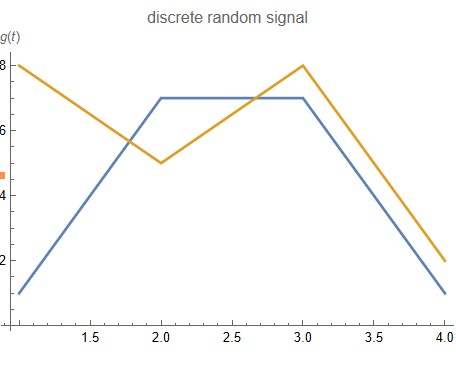
\includegraphics[width=7cm]{images/covariance.jpg}
 \caption{Covariance}
 \label{fig:signal values}
\end{figure}
$$
\begin{aligned}
& x=\{1,7,7,1\} \\
& y=\{8,5,8,2\} \\
& \bar{x} \quad=\frac{1}{N} \sum_{i=1}^N x_i \quad=4.0000 \\
& \bar{y}=\frac{1}{N} \sum_{i=1}^N y_i \quad=5.7500 \\
& \overline{x y}=\frac{1}{N} \sum_{i=1}^N x_i y_i \quad=25.2500 \\
& \hat{\sigma}_x=\sqrt{\frac{1}{N-1} \sum_{i=1}^N\left(x_i-\bar{x}\right)^2}=3.4641 \\
& \hat{\sigma}_y=\sqrt{\frac{1}{N-1} \sum_{i=1}^N\left(y_i-\bar{y}\right)^2}=2.8723 \\
& \hat{\sigma}_{x y}=\frac{\sum_{i=1}^n\left(X_i-\bar{X}\right)\left(Y_i-\bar{Y}\right)}{n-1}=3.0000 \\
& \hat{\rho}=\frac{\hat{\sigma}_{x y}}{\hat{\sigma}_x \hat{\sigma}_y}={0.3015} \\
&
\end{aligned}
$$
\subsubsection{Calculations}
To calculate the next sample in a kalman filter one must know what the following variables mean: 
\begin{itemize}
  \item $\mathbf{F}_k$, the state-transition model;
  \item $\mathbf{H}_k$, the observation model;
  \item $\mathbf{Q}_k$, the covariance of the process noise;
  \item $\mathbf{R}_k$ the covariance of the observation noise;
\end{itemize}



Furthermore one must be familiar with the \href{https://en.wikipedia.org/wiki/State-space_representation}{state space reperesentation}. Thereby the following \href{https://youtu.be/-cD7WkbAIL0}{video series} is very helpful.
For a Kalman-Filter one can use the following recipe:
\begin{enumerate}
  \item Set $k=0$, enter the prior estimate $\hat{\boldsymbol{x}}_{0 \mid-1}$ and an intial value for the erro covariance matrix $\boldsymbol{P}_{0 \mid-1}$
  \item Compute the Kalman gain: $\boldsymbol{k}_k=\boldsymbol{P}_{k \mid k-1} C^T\left(\boldsymbol{C} \boldsymbol{P}_{k \mid k-1} C^T+R_k\right)^{-1}$
  \item Update the estimate with the new measurement $y_k: \hat{\boldsymbol{x}}_{k \mid k}=\hat{\boldsymbol{x}}_{k \mid k-1}+\boldsymbol{k}_k\left(y_k-\boldsymbol{C} \hat{\boldsymbol{x}}_{k \mid k-1}\right)$
  \item Compute the error covariance matrix: $\boldsymbol{P}_{k \mid k}=\left(\boldsymbol{I}-\boldsymbol{k}_k \boldsymbol{C}\right) \boldsymbol{P}_{k \mid k-1}$
  \item Project ahed: $\hat{\boldsymbol{x}}_{k+1 \mid k}=\boldsymbol{A} \hat{\boldsymbol{x}}_{k \mid k}$ and $\boldsymbol{P}_{k+1 \mid k}=\boldsymbol{A} \boldsymbol{P}_{k \mid k} \boldsymbol{A}^T+\boldsymbol{Q}_k$
  \item Increment $k$ and return to step 2.
\end{enumerate}

\begin{equation}\label{eq:kalman_P_kk}
\begin{aligned}
\boldsymbol{P}_{k \mid k} &=E\left\{\left(\boldsymbol{x}_k-\hat{\boldsymbol{x}}_{k \mid k-1}\right)\left(\boldsymbol{x}_k-\hat{\boldsymbol{x}}_{k \mid k-1}\right)^T-\boldsymbol{k}_k e_{k \mid k-1}\left(\boldsymbol{x}_k-\hat{\boldsymbol{x}}_{k \mid k-1}\right)^T\right\} \\
&=\boldsymbol{P}_{k \mid k-1}-\boldsymbol{k}_k \boldsymbol{C} \boldsymbol{P}_{k \mid k-1} \\
&=\left(\boldsymbol{I}-\boldsymbol{k}_k \boldsymbol{C}\right) \boldsymbol{P}_{k \mid k-1} .
\end{aligned}
\end{equation}
\begin{equation}\label{eq:kalman_k_k}
k_k=\boldsymbol{P}_{k \mid k-1} C^T\left(C P_{k \mid k-1} C^T+R_k\right)^{-1}
\end{equation}
\begin{equation}\label{eq:kalman_x_kk}
\hat{\boldsymbol{x}}_{k \mid k}=\hat{\boldsymbol{x}}_{k \mid k-1}+\boldsymbol{k}_k\left(y_k-\boldsymbol{C} \hat{\boldsymbol{x}}_{k \mid k-1}\right)
\end{equation}
\begin{equation}\label{eq:kalman_P_kk+1}
\begin{aligned}
\boldsymbol{P}_{k+1 \mid k} &=E\left\{\left(\boldsymbol{x}_{k+1}-\hat{\boldsymbol{x}}_{k+1 \mid k}\right)\left(\boldsymbol{x}_{k+1}-\hat{\boldsymbol{x}}_{k+1 \mid k}\right)^T\right\} \\
&=E\left\{\boldsymbol{A}\left(\boldsymbol{x}_k-\hat{\boldsymbol{x}}_{k \mid k}\right)\left(\boldsymbol{x}_k-\hat{\boldsymbol{x}}_{k \mid k}\right)^T \boldsymbol{A}^T+\boldsymbol{u}_k \boldsymbol{u}_k^T\right\} \\
&=\boldsymbol{A} \boldsymbol{P}_{k \mid k} \boldsymbol{A}^T+\boldsymbol{Q}_k
\end{aligned}
\end{equation}
\begin{equation}\label{eq:kalman_x_kk_2}
\hat{\boldsymbol{x}}_{k \mid k}=\hat{\boldsymbol{x}}_{k \mid k-1}+\frac{\boldsymbol{P}_{k \mid k-1} \boldsymbol{C}^T}{\boldsymbol{C P _ { k | k - 1 } C ^ { T } + 1}}\left(y_k-\boldsymbol{C} \hat{\boldsymbol{x}}_{k \mid k-1}\right)
\end{equation}
\begin{equation}\label{eq:kalman_x_kk+1}
\boldsymbol{x}_{k+1}=\boldsymbol{A} \boldsymbol{x}_k+\boldsymbol{B} \boldsymbol{u}_k
\end{equation}






\begin{figure}[ht]
 \centering
 %\includestandalone[width=1\linewidth]{kalman.tex} % without the `.tex` extension
 \resizebox{1\textwidth}{!}{\subimport{images/}{kalman.tex}}
 \caption{Kalman example}
 \label{fig:kalman_1}
\end{figure}

\subsubsection{Example Kalman filter}
You are given a linear, shift-invariant system as depicted above. This system has the scalar state $x_k$ and produces
the scalar output $y_k$ at every discrete time instant $k$. The measurement-noise $v_k$ and the process-noise $u_k$ are zero-mean Gaussian random variables with $\textcolor{pink}{R_k} = E\{v_k^2\}=\textcolor{pink}{1}$ and $Q_k = E\{u_k^2\}= 1$.
\begin{figure}[ht]
 \centering
 %\includestandalone[width=1\linewidth]{kalman_example.tex} % without the `.tex` extension
 \resizebox{1\textwidth}{!}{\subimport{images/}{kalman_example.tex}}
 \caption{Kalman example}
 \label{fig:kalman_example}
\end{figure}


$$
\begin{array}{|c|c|c|c|}
\hline k & P_{k \mid k-1} & k_k & P_{k \mid k} \\
\hline 0 & \textcolor{blue}{\frac{4}{3}} & & \\
1 & & & \\
2 & & & \\
\hline
\end{array}
$$

$$
\begin{array}{|r|r|r|r|}
\hline k & y_k & \hat{x}_{k \mid k-1} & \hat{x}_{k \mid k} \\
\hline 0 & \textcolor{orange}{0.80} & \textcolor{brown}{0.00} & \\
1 & -1.20 & & \\
2 & 0.10 & & \\
\hline
\end{array}
$$

$$
\begin{array}{|c|c|c|c|}
\hline k & P_{k \mid k-1} & k_k & P_{k \mid k} \\
\hline 0 & 0 & & \\
1 & & & \\
2 & & & \\
\hline
\end{array}
$$

First one has to calculate $k_k$ which can be done with \autoref{eq:kalman_k_k}. From \autoref{fig:kalman_1} we know that $C=1$, $\textcolor{blue}{P_{k \mid k-1}}=\textcolor{blue}{\frac{4}{3}}$ and $R_k=1$. Therefore
$$
\textcolor{violet}{\boldsymbol{k}_k}=\textcolor{blue}{\boldsymbol{P}_{k \mid k-1}} C^T\left(\boldsymbol{C} \textcolor{blue}{\boldsymbol{P}_{k \mid k-1}} C^T+\textcolor{pink}{R_k}\right)^{-1}=\textcolor{blue}{\frac{4}{3}} \cdot 1 \cdot \left(1\cdot \textcolor{blue}{\frac{4}{3}}\cdot 1 +\textcolor{pink}{1} \right)^{-1}=\textcolor{violet}{\frac{4}{7}}
$$
In the next step one can calculate $\hat{x}_{k \mid k}$ with the new measurement $y_k$, therefore and due to \autoref{eq:kalman_x_kk}
$$
\textcolor{olive}{\hat{\boldsymbol{x}}_{k \mid k}}=\textcolor{brown}{\hat{\boldsymbol{x}}_{k \mid k-1}}+\textcolor{violet}{\boldsymbol{k}_k}\left(y_k-\boldsymbol{C} \hat{\boldsymbol{x}}_{k \mid k-1}\right)=\textcolor{brown}{0}+\textcolor{violet}{\frac{4}{7}}\cdot \left(\textcolor{orange}{\frac{4}{5}} - 1 \cdot \textcolor{brown}{0} \right)=\textcolor{olive}{\frac{16}{35}}
$$
With \autoref{eq:kalman_P_kk} one can now calculate $P_{k \mid k}$.
$$
\textcolor{teal}{\boldsymbol{P}_{k \mid k}}=\left(\boldsymbol{I}-\textcolor{violet}{\boldsymbol{k}_k} \boldsymbol{C}\right) \textcolor{blue}{\boldsymbol{P}_{k \mid k-1}}=\left(1-\textcolor{violet}{\frac{4}{7}}\cdot 1 \right) \cdot \textcolor{blue}{\frac{4}{3}}=\textcolor{teal}{\frac{4}{7}}
$$
In the next step, one can calculate $\textcolor{magenta}{\boldsymbol{P}_{k+1 \mid k}}$ with \autoref{eq:kalman_P_kk+1}
$$
\textcolor{magenta}{\boldsymbol{P}_{k+1 \mid k}}=\textcolor{red}{\boldsymbol{A}} \textcolor{teal}{\boldsymbol{P}_{k \mid k}} \textcolor{red}{\boldsymbol{A}}^T+\boldsymbol{Q}_k=\textcolor{red}{\frac{1}{2}}\cdot \textcolor{teal}{\frac{4}{7}} \cdot \textcolor{red}{\frac{1}{2}} +1=\textcolor{magenta}{\frac{8}{7}}
$$
With \autoref{eq:kalman_x_kk+1} one can calculate $\boldsymbol{x}_{k+1}$
$$
\hat{\boldsymbol{x}}_{k+1 \mid k}=\textcolor{red}{\boldsymbol{A}} \textcolor{olive}{\hat{\boldsymbol{x}}_{k \mid k}}=\textcolor{red}{\frac{1}{2}}\cdot \textcolor{olive}{\frac{16}{35}}=\frac{8}{35}
$$
Now one can repeat the steps before and one gets the following result:
$$
\begin{array}{|c|c|c|c|}
\hline k & P_{k \mid k-1} & k_k & P_{k \mid k} \\
\hline 0 & \textcolor{blue}{\frac{4}{3}} & \textcolor{violet}{\frac{4}{7}} & \textcolor{teal}{\frac{4}{7}} \\
1 & \textcolor{magenta}{\frac{8}{7}} & \frac{8}{15} & \frac{8}{15} \\
2 & \frac{17}{15} & \frac{17}{32} & \frac{17}{32} \\
\hline
\end{array}
$$




Now one can repeat the steps before and one gets the following result:

$$
\begin{array}{|r|r|r|r|}
\hline k & y_k & \hat{x}_{k \mid k-1} & \hat{x}_{k \mid k} \\
\hline 0 & \textcolor{orange}{0.80} & \textcolor{brown}{0.00} & \textcolor{olive}{\frac{16}{35}} \\
1 & -1.20 & \frac{8}{35} & -0.53 \\
2 & 0.10 & -0.27 & -0.07 \\
\hline
\end{array}
$$

$$
\begin{array}{|c|c|c|c|}
\hline k & P_{k \mid k-1} & k_k & P_{k \mid k} \\
\hline 0 & 0 & 0 & 0 \\
1 & 1 & \frac{1}{2} & \frac{1}{2} \\
2 & \frac{9}{8} & \frac{9}{17} & \frac{9}{17} \\
\hline
\end{array}
$$
Alternatively, one can also program a \href{https://youtu.be/x0-NaGaCzew}{program} on the ti-nspire and call it then like the following:
\begin{verbatim}
sign_proc\kalman(1,1,((4)/(3)),0,[((1)/(2))],[1],[1],((4)/(5)))
\end{verbatim}
sign\_proc\textbackslash kalman($R_k$,$Q_k$,$P_{k|k-1}$,$x_{k|k-1}$,$A$,$B$,$C$,$y_k$)\newline
which outputs then the following:\newline
$R_k: 1 , Q_k: 1 , P_{k|k-1}: ((4)/(3)) , x_{k|k-1}: 0 , A: [((1)/(2))] , B: [1] , C: [1] , y_k: ((4)/(5))$
$k_k= [(\textcolor{violet}{(4)/(7)})] , \hat{x}_{k_k}= [(\textcolor{olive}{(16)/(35)})] , p_{k|k}= [(\textcolor{teal}{(4)/(7)})] , x_{k+1|k}= [((8)/(35))] , p_{k+1|k}= [(\textcolor{pink}{(8)/(7)})]$\newline
The program itself looks like the following:
\begin{verbatim}
Define LibPub kalman(r_k,q_k,pkk_m_1,xkk_m_1,a,b,c,y_k)=
Prgm
:©Inputs a(R_k (covariance of observation noise), R_k (covariance of the proccess noise), pkk_m_1,xkk_m_1, a,b,c,y_k)
:Disp "R_k: ",r_k,", Q_k: ",q_k,", P_{k|k-1}: ",pkk_m_1,", x_{k|k-1}: ",xkk_m_1," , A: ",a," , B: ",b," , C: ",c," , y_k: ",y_k
:Disp " "
:Local k_k,x_k_k,p_k_k,xkk_p_1,pkk_p_1
:k_k:=pkk_m_1*c^T*(c*pkk_m_1*c^T+r_k)^(-1)
:x_k_k:=xkk_m_1+k_k*(y_k-c*xkk_m_1)
:p_k_k:=(identity(max(dim(c)))-k_k*c)*pkk_m_1
:xkk_p_1:=a*x_k_k
:pkk_p_1:=a*p_k_k*a^T+q_k
:Disp "k_k=",k_k," , \hat{x}_{k_k}=",x_k_k," , p_{k|k}=",p_k_k," , x_{k+1|k}=",xkk_p_1," , p_{k+1|k}=",pkk_p_1
:PassErr
:EndPrgm
\end{verbatim}

\subsubsection{Example 2}
Lets assume we want to measure the position of an airplane, with $v_{0 x}=280$ and $x_0=4000\mathrm{~m}$.
\paragraph{Observations}
$$
\begin{array}{ll}
x_0=4000 \mathrm{~m} & v_{0 x}=280 \mathrm{~m} / \mathrm{sec} \\
x_1=4260 \mathrm{~m} & v_{1 x}=282 \mathrm{~m} / \mathrm{sec} \\
x_2=4550 \mathrm{~m} & v_{2 x}=285 \mathrm{~m} / \mathrm{sec} \\
x_3=4860 \mathrm{~m} & v_{3 x}=286 \mathrm{~m} / \mathrm{ser} \\
x_4=5110 \mathrm{~m} & v_{4 x}=290 \mathrm{~m} / \mathrm{sec}
\end{array}
$$
\paragraph{Initial Conditions}
$$
\begin{array}{ll}
a_x=2 \mathrm{~m} / \mathrm{sec}^2 & \Delta t=1 \mathrm{sec} \\
V_x=280 \mathrm{~m} / \mathrm{sec} & \Delta x=25 \mathrm{~m}
\end{array}
$$
\paragraph{Process Errors i Process covariance matrix}
$$
\begin{aligned}
&\Delta P_x=20 \mathrm{~m} \\
&\Delta P_{v_x}=5 \mathrm{~m} / \mathrm{sec}
\end{aligned}
$$
\paragraph{Observations errors}
$$
\begin{aligned}
&\Delta x=25 \mathrm{~m} \\
&\Delta v_x=6 \mathrm{~m} / \mathrm{sec}
\end{aligned}
$$
Our estimate of $X_{k_p}$ which is the next state is the following:
$$
\begin{aligned}
X_{k_p} &=A X_{k-1}+B u_k+w_k \\
&=\left[\begin{array}{ll}
1 & \Delta t \\
0 & 1
\end{array}\right]\left[\begin{array}{c}
x_0 \\
v_0
\end{array}\right]+\left[\begin{array}{c}
\frac{1}{2} \Delta t^2 \\
\Delta t
\end{array}\right]\left[a_{x_0}\right]+0 \\
&=\left[\begin{array}{ll}
1 & 1 \\
0 & 1
\end{array}\right]\left[\begin{array}{c}
4000 \\
280
\end{array}\right]+\left[\begin{array}{c}
1 / 2 \\
1
\end{array}\right]\left[\begin{array}{l}
2
\end{array}\right] \\
&=\left[\begin{array}{c}
4280 \\
280
\end{array}\right]+\left[\begin{array}{l}
1 \\
2
\end{array}\right] \\
X_{k_p} &=\left[\begin{array}{c}
4281 \\
282
\end{array}\right]
\end{aligned}
$$
\paragraph{Initial Process Covariance}
The cross term is often set to zero, since they are independent of each other.
$$
\begin{aligned}
&P_{k-1}=\left[\begin{array}{cc}
\Delta x^2 & \Delta x \Delta v \\
\Delta x \Delta v & \Delta v_x^2
\end{array}\right]=\left[\begin{array}{ll}
400 & 100 \\
100 & 25
\end{array}\right] \\
&P_{k-1}=\left[\begin{array}{cc}
400 & 0 \\
0 & 25
\end{array}\right]
\end{aligned}
$$
\paragraph{The predicted process covariance matrix}
$$
\begin{aligned}
P_{k p} &=A P_{k-1} A^{\top}+Q_R \\
&=\left[\begin{array}{ll}
1 & \Delta t \\
0 & 1
\end{array}\right]\left[\begin{array}{cc}
400 & 0 \\
0 & 25
\end{array}\right]\left[\begin{array}{ll}
1 & 0 \\
\Delta t & 1
\end{array}\right]+0 \\
&=\left[\begin{array}{ll}
1 & 1 \\
0 & 1
\end{array}\right]\left[\begin{array}{cc}
400 & 0 \\
0 & 25
\end{array}\right]\left[\begin{array}{ll}
1 & 0 \\
1 & 1
\end{array}\right] \\
&=\left[\begin{array}{cc}
400 & 25 \\
0 & 25
\end{array}\right]\left[\begin{array}{ll}
1 & 0 \\
1 & 1
\end{array}\right] \\
&=\left[\begin{array}{ll}
425 & 25 \\
25 & 25
\end{array}\right] \Rightarrow\left[\begin{array}{cc}
425 & 0 \\
0 & 25
\end{array}\right]
\end{aligned}
$$
\paragraph{Calculating the Calman Gain}
$$
\begin{aligned}
K &=\frac{P_{k_p} H^{\top}}{H P_{k_p} H^{\top}+R} \\
&=\frac{\left[\begin{array}{cc}
425 & 0 \\
0 & 25
\end{array}\right]\left[\begin{array}{ll}
1 & 0 \\
0 & 1
\end{array}\right]}{\left[\begin{array}{ll}
1 & 0 \\
0 & 1
\end{array}\right]\left[\begin{array}{cc}
425 & 0 \\
0 & 25
\end{array}\right]\left[\begin{array}{ll}
1 & 0 \\
0 & 1
\end{array}\right]+\left[\begin{array}{cc}
625 & 0 \\
0 & 36
\end{array}\right]} \\
&=\frac{\left[\begin{array}{cc}
425 & 0 \\
0 & 25
\end{array}\right]}{\left[\begin{array}{cc}
425 & 0 \\
0 & 25
\end{array}\right]+\left[\begin{array}{cc}
625 & 0 \\
0 & 36
\end{array}\right]}=\frac{\left[\begin{array}{cc}
425 & 0 \\
0 & 25
\end{array}\right]}{\left[\begin{array}{cc}
1050 & 0 \\
0 & 61
\end{array}\right]}=\left[\begin{array}{cc}
0.405 & 0 \\
0 & 0.410
\end{array}\right]
\end{aligned}
$$
\paragraph{The new Observation}
$$
\begin{aligned}
&Y_k=C y_k+Z_k \\
&Y_k=\left[\begin{array}{ll}
1 & 0 \\
0 & 1
\end{array}\right]\left[\begin{array}{c}
4260 \\
282
\end{array}\right]+0 \\
&Y_k=\left[\begin{array}{l}
4260 \\
282
\end{array}\right]
\end{aligned}
$$
\paragraph{Calculate the current state}
$$
\begin{aligned}
&X_k=X_{k_p}+K\left[Y_k-H X_{k_p}\right]\\
&=\left[\begin{array}{l}
4281 \\
282
\end{array}\right]+\left[\begin{array}{cc}
0.405 & 0 \\
0 & 0.410
\end{array}\right]\left(\left[\begin{array}{l}
4260 \\
282
\end{array}\right]-\left[\begin{array}{cc}
1 & 0 \\
0 & 1
\end{array}\right]\left[\begin{array}{ll}
4281 \\
282
\end{array}\right]\right)\\
&=\left[\begin{array}{c}
4281 \\
282
\end{array}\right]+\left[\begin{array}{cc}
0.405 & 0 \\
0 & 0.410
\end{array}\right]\left[\begin{array}{c}
-21 \\
0
\end{array}\right]\\
&=\left[\begin{array}{c}
4281 \\
282
\end{array}\right]+\left[\begin{array}{c}
-8.5 \\
0
\end{array}\right]\\
&X_k=\left[\begin{array}{c}
4272.5 \\
282
\end{array}\right]
\end{aligned}
$$
\paragraph{Update Process Covariance}
$$
\begin{aligned}
&P_k=(I-K H) P_{k_p}\\
&P_k=\left[\left[\begin{array}{ll}
1 & 0 \\
0 & 1
\end{array}\right]-\left[\begin{array}{cc}
0.405 & 0 \\
0 & 0.410
\end{array}\right]\left[\begin{array}{ll}
1 & 0 \\
0 & 1
\end{array}\right]\left[\begin{array}{cc}
425 & 0 \\
0 & 25
\end{array}\right]\right.\\
&P_k=\left[\left[\begin{array}{ll}
1 & 0 \\
0 & 1
\end{array}\right]-\left[\begin{array}{cc}
0.405 & 0 \\
0 & 0.410
\end{array}\right]\left[\begin{array}{cc}
425 & 0 \\
0 & 25
\end{array}\right]\right.\\
&k=\left[\begin{array}{cc}
0.595 & 0 \\
0 & 0.590
\end{array}\right]\left[\begin{array}{cc}
425 & 0 \\
0 & 25
\end{array}\right]\\
&P_k=\left[\begin{array}{cc}
253 & 0 \\
0 & 14.8
\end{array}\right]
\end{aligned}
$$
\paragraph{Current Becomes previous}
$$
\begin{aligned}
&X_k=\left[\begin{array}{c}
4272.5 \\
282
\end{array}\right] \Rightarrow X_{k-1} \Rightarrow X_{k_p}=A X_{k-1}+B_k+w_k \\
&P_k=\left[\begin{array}{cc}
253 & 0 \\
0 & 14.8
\end{array}\right] \Rightarrow P_{k-1} \Rightarrow P_{k_p}=A P_{k-1} A^{\top}+Q_k
\end{aligned}
$$